\documentclass[11pt]{report}
\usepackage{fullpage}
\usepackage[pdftex,
            pdfauthor={Jeffrey Yoo Warren},
            pdftitle={Grassroots Mapping: a toolkit for participatory and activist cartography},
            pdfsubject={Participatory Cartography},
            pdfkeywords={Cartography},
            pdfproducer={Latex with hyperref},
            pdfcreator={pdflatex,colorlinks}]{hyperref}
\usepackage{graphicx,wrapfig,color}
\definecolor{linkblue}{rgb}{0.2,0.2,1}
\hypersetup{colorlinks=true,
	    urlcolor=linkblue}

\title{Grassroots Mapping: a toolkit for participatory and politically engaged cartography}
\author{Jeffrey Warren}
\date{May 7, 2010}

%% Define a new 'leo' style for the package that will use a smaller font.
\makeatletter
\def\url@jeffstyle{%
  \@ifundefined{selectfont}{\def\UrlFont{\sf}}{\def\UrlFont{\small\ttfamily}}}
\makeatother
%% Now actually use the newly defined style.
\urlstyle{jeff}

\begin{document}
\maketitle

\chapter{Introduction}
\section{Overview}
\section{Defining Grassroots Mapping: Toolkit, Practices, or Community?}

Exactly what makes up the Grassroots Mapping project? Is it a body of code, available under an MIT license at \url{http://github.com/jywarren/cartagen}? Is it a set of mapping practices, or tools, which have been employed in Lima, Peru, or Rio de Janiero? Or is it a community of practitioners and the web site, wiki, and mailing list which tie them together?

\subsection{Software}
\subsubsection{Interfaces for participatory cartography}
\subsubsection{The Cartagen framework}
\subsubsection*{Rendering architecture}
\subsection{Practice, Community, Support structure}
\subsubsection{GrassrootsMapping.org}
\subsubsection*{The Grassroots Mapping Wiki}
\begin{wrapfigure}{r}{0.5\textwidth}
	\begin{flushright}
		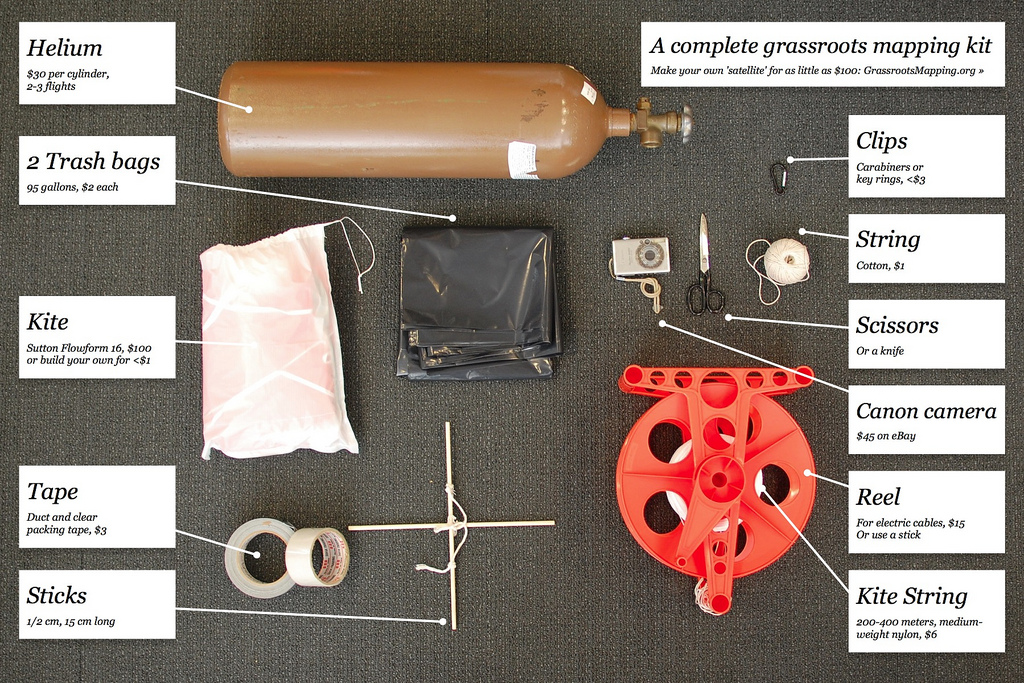
\includegraphics[width=0.45\textwidth]{images/100-dollar-satellite-poster.jpg}
	\end{flushright}
\end{wrapfigure}
\subsubsection*{Documentation, case studies, Grassroots Map Collection}
\subsubsection*{The Grassroots Mapping community and mailing list}
\section{Novel Contributions}
\subsection{Novel application of low-cost tools to well-established need for raster imagery}
%do we discuss existing systems here? no, just mention paradigms of tiles, reference later section
\subsection{Novel approaches to map rendering}
\subsection{Central merit: technology or culture?}
%both, duh: technology is only relevant in a context, and I make no attempt to separate this technology from its intended sociopolitical meaning

\chapter{Subjectivity in Mapping}
\section{The mythical 'complete' map}
%We often imagine 'complete maps'
% Epistomology and mapping: maps are a form of technology, and of power      
%  - OSM reference to a 'complete map of UK'
%        - Chris Anderson's Wired article of complete dataset
\section{Maps: rhetorical, even tactical}
%        - Endless variety of possible data: Wood, Power of Maps, p.1
%        - not a representation of truth, but a rhetorical tool; Wood, p1?
%            - social construction of maps
% 	- map of sewer system from Wood
%	- Tactical cartography from Institute for Applied Autonomy
\section{Ground Truth, or maps as testimony}
%    - varying definitions of ownership, contested terrain
%        - 'Ground Truth' policy in OSM (http://wiki.openstreetmap.org/wiki/Disputes#On_the_Ground_Rule)
\subsection{Subjective cartography in practice}
%    - ref. West Bank mapping in Dec 2009
% Tree symbolism
% B'Tselem map of settlements
%        - mapping as testimony of use/presence/ownership by Abed's farm


\chapter{The Need for Geospatial Data}
\section{Two worlds of mapping}
\subsection{Urban slums, informal settlements}
%    UN-HABITAT quotation
\subsection{Tenure mapping}
\subsubsection{The invasion of Lima, Peru}
%        - El Otro Sendero
%            - graph of informal settlement percentages
%        - COFOPRI
\section{Environmental assessment}
\subsection{Carbon cowboys}
\section{Open geodata and crisis mapping}
\subsection{Crisis mapping and Ushahidi}
%	- origin in political mapping, focus on natural disaster
%        - UN-SPIDER/Google MapMaker response to Mikel Maron, Chile Earthquake

\chapter{State of the Art}
\section{PGIS: Participatory Geographic Information Systems}

Traditional GIS technology has been used since the XX's to support communities in developing contexts for purposes such as making tenure claims, environmental defense against petroleum and other extraction industries, as well as for planning purposes. This has become known as PGIS, or Participatory GIS, and typically... 

\subsection{Participatory GIS for Development}
% Jen Osha's article
%\href{http://www.directionsmag.com/article.php?article_id=2365&trv=1.}{Participatory GIS - A Paradigm Shift in Development?} - Jen Osha and Daniel Weiner, 2006
%        THE ILLUSTRATED GUIDE TO NONPROFIT GIS AND ONLINE MAPPING: http://maptogether.org/nonprofit-mapping
%        Claudia Canepa's PhD dissertation
\subsection{Shortcomings of traditional PGIS practice}
%    Peter Poole - Life after Tenure Mapping
%        - outsourcing of GIS processing typical, problems
\section{OpenStreetMap}

% OSM acronym

\subsection{Humanitarian OSM Team}
%   HOT acronym
\subsubsection{Free Map Gaza}
%        Map Kibera, Free Map Palestine, Free Map India
\subsubsection{Followup projects}
%        Data modeling: http://wiki.openstreetmap.org/wiki/Humanitarian_OSM_Tags/Humanitarian_Data_Model
\subsubsection{Challenges}
%        Slum mapping, disaster-specific issues
%        architectural/infrastructural shortcomings
%	reliance on GPS, or need for a base layer
% 	inclusion in a GPS-device process
%	ease of use, black-boxing of information
%	JOSM, other issues with typical deployment
\textbf{Emphasis on local infrastructure}

\chapter{Grassroots Mapping as an alternative means of participatory cartography}
%    Meet subjectivity needs
%        - against a canonical datastore
%        - solution lays in tools and formats and practices, not in a single project/datastore
%            - therefore GM & Cartagen are based around:
%                - a body of code
%                - a thorough documentation and guide to mapping techniques
%        - options to organize project: as a 'generic hub' for imagery, like OpenAerialMap, engage primarily via internet/blogs
%            - or, focus on collaborating with specific communities in cartographic dispute
%                - expand into matchmaking between mappers and communities in need, as well as supporting via mailing list 
%                - maintain open communication with end-users, iterate back into tools: 
%                    - requests made via list: stewart long asks for masking, Crispen asks for entry of lat/lon pairs, WhereCamp folks asked for locking, Pat Coyle asked for 'natural_size' feature
\section{Cartagen: an alternative architecture}
%        - existing solutions based around cloud systems
%            - this move opposite - closer to client
%            - needs: data under no connectivity
%            - multiple devices
%            - ownership of data/infrastructure
%                - FrontlineSMS, 'local' is a feature, opposite of corporate/commercial strategy
%        - low-AI approach; technical literacy, flexibility, admits 'misuse'
%            - examples: USGS overlay at WhereCamp 2010
%            - additon of non-map features with Warper tool
%            - difficulty of use of hugin, etc
%                - DIYDrones thread: "3 days stitching and tweaking images" (http://diydrones.com/profiles/blog/show?id=705844:BlogPost:134855&page=1#comments)
%            - Stewart Long uses Photoshop for most stitches (get him on record)
%Emphasis on building in response to end-user needs
%    - this work could only be done by working with communities in cartographic dispute. See Lima case study.

\chapter{Related works}
%    Inspiration, context, history of activist/grassroots mapping
%    Reiterate HOT/Free Map Palestine, India, Kibera
%    GroundTruth, Jai Sen, A People's Atlas of Chicago
\section{Beyond symbolic mapping: Data-driven approaches to participatory mapping}
%        Expanding role of mapping to legal, tactical
%        Institute for Applied Autonomy

\chapter{Evaluation criteria}
\section{Participants vs. collaborators}
%        Role of Carla, Escuelab, Shuawa
%        Hector as a fellow educator (interview)
%    'Reconceptualizing Validity' (Patti Lather, p.67)
%        Triangulation
%        Construct validity - how theory was affected by data
%        Face validity - how research was received by participants
%        Catalytic Validity - how participation transforms the situation (self-awareness/reflexivity)
%    Interview process
%    Wiki, mailing list, blog, media coverage (~ Face validity)

\chapter{The Grassroots Mapping tool chain}
\section{Balloon/kite Aerial Mapping (BAM/KAM)}
%    UAV - DIYDrones and collaboration (see 'Future work')
%        Leveraging both expert and 'amateur'/enthusiast expertise
%        Connecting hobby/DIY communities with activist communities and agendas
\section{Digital maps: reconceptualizing mapping interaction}
\subsection{Beyond raster mapping/Tile politics}
%            Metadata: authorship data
%            Google Maps png metadata hack
%            GIS and broadly adopted consumer-focused mapping stacks
\subsection{Cartagen dynamic rendering}
%            Existing vector systems (Chris Schmitt's email on geowanking)
%            Limitations: technical, barrier-to-entry, participatory, literacy
%                GSS (and OSM-JSON): appropriating the HTML/CSS paradigm for data legibility and open access
%                    Format politics: XML, JSON, RSS
\subsection{An iterative toolchain development process}
%    Toolchain not developed in vacuum, but through collaboration and study on-site
%        - initial flight testing with Josh Levinger
%            - MIT map
%            - terrain, difficulty
%            - optimization for site: Peru, low buildings, no trees
%        - Peru, West Bank, India
%        - Following chapters document those collaborations and their fruits




\begin{figure}[h]
  \begin{center}
    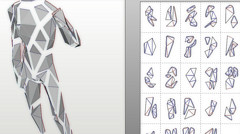
\includegraphics[scale=0.75]{images/test.jpg}
    \caption{The Toucan}
  \end{center}
\end{figure}

\chapter{ReadingList}

\hypertarget{related_readings_1}{}\subsection*{{Related readings}}\label{related_readings_1}

A collection of readings on kids, playful exploration, and grassroots mapping

\textbf{Jeff:}

\href{http://dspace.mit.edu/handle/1721.1/33012}{New information technologies in the old political economy : an exploration of community-based GIS for improving basic services for the poor in New Delhi, India} - 2005 MIT DUSP dissertation by Claudia Canepa

\href{http://www.ejisdc.org/ojs2/index.php/ejisdc/article/viewFile/237/158}{PARTICIPATORY SPATIAL INFORMATION MANAGEMENT AND COMMUNICATION IN DEVELOPING COUNTRIES} - Giacomo Rambaldi, Peter A Kwaku Kyem, Mike $\backslash$McCall, Daniel Weiner, EJISDC, 2006

\href{http://books.google.com/books?id=4u79ffyzekoC&printsec=frontcover&dq=child%27s+pictorial+world&ei=5EUYS9veGqPqygShs7TVBw#v=onepage&q=&f=false}{The child'{}s creation of a pictorial world}, Claire Golomb

\href{http://www.unicef.org/teachers/researchers/intro.htm}{Curriculum on ``{}Children as Community Researchers''{}} - UNICEF, authored by \href{http://web.gc.cuny.edu/che/cerg/about_cerg/environmental_learning_index.htm}{Children'{}s Environment Research Group}

\href{http://www.directionsmag.com/article.php?article_id=2365&trv=1.}{Participatory GIS - A Paradigm Shift in Development?} - Jen Osha and Daniel Weiner, 2006

\href{http://www.iapad.org/pgis2005/}{Mapping for Change} - 2005 International Conference on Participatory Spatial Information Management and Communication

Weiner, D. and T. Harris, 2003. ''{}\href{http://www.rri.wvu.edu/pdffiles/gisweiner.pdf}{Community-Integrated GIS for Land Reform in South Africa}.''{} URISA Journal. 15(2): 61-73.

\href{http://www.maptogether.net/taxonomy/term/151}{PPGIS on MapTogether.net}

\href{http://books.google.com/books?hl=en&lr=&id=_VK-ABCKlVgC&oi=fnd&pg=PA3&dq=Nino+Bariola&ots=_r1wMwjiou&sig=TH0Gn1P27Xtsdq2Oc0Up5D6HLzg#v=onepage&q=Nino%20Bariola&f=false}{Bilingualism and identity: Spanish at the crossroads with other languages} - Geographic dispute in Canta Gallo, in Lima, \href{http://books.google.com/books?id=_VK-ABCKlVgC&lpg=PA3&ots=_r1wMwjiou&dq=Nino%20Bariola&lr=&pg=PA153#v=onepage&q=&f=true}{Chapter 7}

\href{http://www.sciencedirect.com/science?_ob=ArticleURL&_udi=B6VG2-4XHJX4B-1&_user=10&_coverDate=08/31/2009&_rdoc=1&_fmt=high&_orig=search&_sort=d&_docanchor=&view=c&_searchStrId=1186930669&_rerunOrigin=google&_acct=C000050221&_version=1&_urlVersion=0&_userid=10&md5=a9327ffa62e089e863f892a4551c1717}{Intervention: Mapping is critical!} - This intervention targets the much heralded demise of the map in geography and the recently proposed “rethinking” of maps. It comprises contributions from two political geographers, a military geographer, a political scientist, and two activist cartographers and argues that there is not so much a need to “rethink” maps, but to “re-engage” with the material practices of mapping, and above all to “re-make” maps.

\href{http://training.esri.com/campus/library/bibliography/RecordDetail.cfm?ID=95545&browseonly=0}{Mapping in a Shoebox} - A Grassroots Approach for Developing the Geospatial Literacy of Elementary Children - 24th International Cartographic Conference - Jaqueline M. Anderson, Sally Hermansen, Lorraine Innes, 2009

Lots of work by Proboscis: \href{http://urbantapestries.net/}{Social Tapestries/Urban Tapestries}, 2002-7 - Urban Tapestries investigated how, by combining mobile and internet technologies with geographic information systems, people could `{}author'{} the environment around them; a kind of Mass Observation for the 21st Century. Like the founders of Mass Observation in the 1930s, we were interested creating opportunities for an ``{}anthropology of ourselves''{} – adopting and adapting new and emerging technologies for creating and sharing everyday knowledge and experience; building up organic, collective memories that trace and embellish different kinds of relationships across places, time and communities.

\href{http://www.geoconnections.org/publications/Key_documents/Sensitive_Env_Geo_Data_Guide_EN_v1.pdf}{BEST PRACTICES FOR SHARING SENSITIVE ENVIRONMENTAL GEOSPATIAL DATA} - for GeoConnections by AMEC Earth \& Environmental, 2010

\textbf{Kate:}

\href{http://news.bbc.co.uk/2/hi/uk_news/8216071.stm}{BBC article} - train station hires a Director of Fun!

\href{http://www.rajworks.com/index1.htm}{Place-Logging} - MIT thesis

\href{http://www.youtube.com/watch?v=U2uH-jrsSxs&feature=rec-LGOUT-exp_fresh+div-1r-3-HM}{Tube iphone app} - augmented reality

\end{document}
